```latex
\documentclass{tietreport}

% Prevent blank pages before chapters
\let\cleardoublepage\clearpage

\usepackage{graphicx}

\usepackage{graphicx}

% Bibliography
\usepackage[
  date=year,
  style=alphabetic,
  backend=biber,
  sorting=nty,
  maxnames=5,
  minnames=3,
  maxalphanames=4,
  minalphanames=3,
  backref=true,
  doi=false,
  isbn=false,
  url=false,
  eprint=false
]{biblatex}

\addbibresource{references.bib}

% ==================================================
% TITLE PAGE
% ==================================================

\TitlePageHeader{%
  UCS503 - Software Engineering
}

\ProjectTitle{%
  GATED: Apartment Tracker
}

\ProjectSubTitle{%
  A Smart Digital Platform for Apartment and Society Management
}

\author{%
  \texttt{1024030101} Khushi Dangi \\
  \texttt{1024030115} Geetika Parakh \\
  \texttt{1024030121} Ridham Sharma \\
  \texttt{1024030937} Harnoor Singh
}

\TitlePageSubText{%
  Group: \texttt{3C14} \\
  BE Third Year, CSE
}

\AdvisorName{%
  Dr. Anushka
}

\TitlePageFooterText{{%
    \large Mid-Semester Evaluation \\[0.2cm]
    \bfseries Computer Science and Engineering Department
  } \\[0.15cm]
  Thapar Institute of Engineering and Technology, Patiala%
}

% ==================================================

\begin{document}

\maketitle

\tableofcontents

% ==================================================
% CHAPTER 1
% ==================================================

\chapter{Introduction}

\section{Background}

Apartment and residential society management involves
residents, society administrators, security guards, and
maintenance staff. Many societies still depend on manual
registers, phone calls, and messaging applications for
managing visitors, maintenance requests, and
communication.

GATED: Apartment Tracker is a mobile application designed
to provide a centralized platform for managing
day-to-day activities within an apartment society.

The system connects residents, society administrators,
security guards, and maintenance staff through
role-based access.

\section{Problem Statement}

Traditional apartment management systems often rely on
manual and disconnected processes. Visitor information
may be maintained in physical registers, maintenance
complaints may be communicated through calls or messages,
and residents may have no centralized method to track
their requests.

Security personnel also require an efficient way to
verify visitors, while society administrators need a
centralized system to manage residents and society
activities.

Therefore, GATED: Apartment Tracker aims to provide a
centralized digital solution for apartment management,
visitor access, maintenance tracking, and communication.

\section{Project Objectives}

\begin{enumerate}
    \item Provide a centralized platform for apartment
    society management.

    \item Implement role-based access for residents,
    society administrators, security guards, and
    maintenance staff.

    \item Allow residents to register, log in, and
    access society services.

    \item Enable residents to raise and track
    maintenance requests.

    \item Allow security personnel to manage visitor
    access.

    \item Provide administrators with centralized
    control over society activities.

    \item Maintain secure user and society data.
\end{enumerate}

% ==================================================
% CHAPTER 2
% ==================================================

\chapter{Methodology and Design}

\section{System Architecture}

GATED: Apartment Tracker follows a client-server
architecture. The mobile application acts as the client
and communicates with the backend for authentication and
database operations.

The system uses role-based access control. After
authentication and society selection, users are directed
to functionality according to their assigned role.

\subsection{System Components}

The major components of the system are:

\begin{itemize}
    \item \textbf{Resident Module:} Provides access to
    society services, maintenance requests, and visitor
    management.

    \item \textbf{Society Admin Module:} Provides
    administrative control over society activities and
    residents.

    \item \textbf{Security Module:} Handles visitor
    verification and access management.

    \item \textbf{Maintenance Module:} Handles
    maintenance requests raised by residents.

    \item \textbf{Authentication Module:} Handles
    registration and login.

    \item \textbf{Database Module:} Stores users,
    societies, apartments, maintenance requests, and
    visitor-related information.
\end{itemize}

\subsection{Application Flow}

\begin{center}
Registration
$\rightarrow$
Login
$\rightarrow$
Society Selection
$\rightarrow$
Role Verification
$\rightarrow$
Role-Based Dashboard
\end{center}

% ==================================================
% USE CASE DIAGRAM
% ==================================================

\section{Use Case Diagram}

The Use Case Diagram represents the interaction between
the four major actors of the system and the
functionalities provided by GATED: Apartment Tracker.

\begin{figure}[htbp]
    \centering
    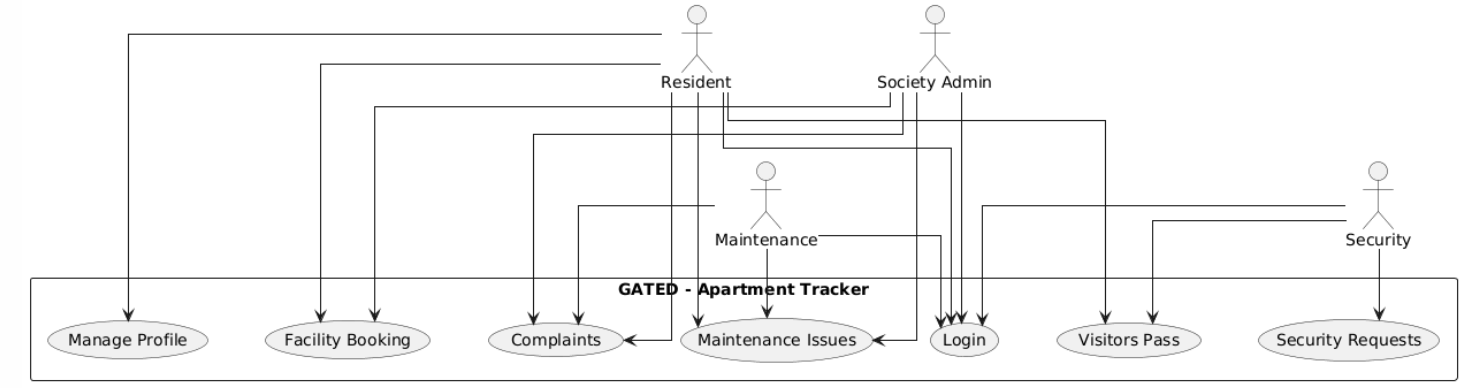
\includegraphics[width=0.95\textwidth]{use_case_diagram.png}
    \caption{Use Case Diagram of GATED: Apartment Tracker}
    \label{fig:usecase}
\end{figure}

The major actors are Resident, Society Admin, Security,
and Maintenance Staff. Each actor has access to
functionality according to their role.

% ==================================================
% UML CLASS DIAGRAM
% ==================================================

\section{UML Class Diagram}

The UML Class Diagram represents the main software
entities and their relationships within the application.

\begin{figure}[htbp]
    \centering
    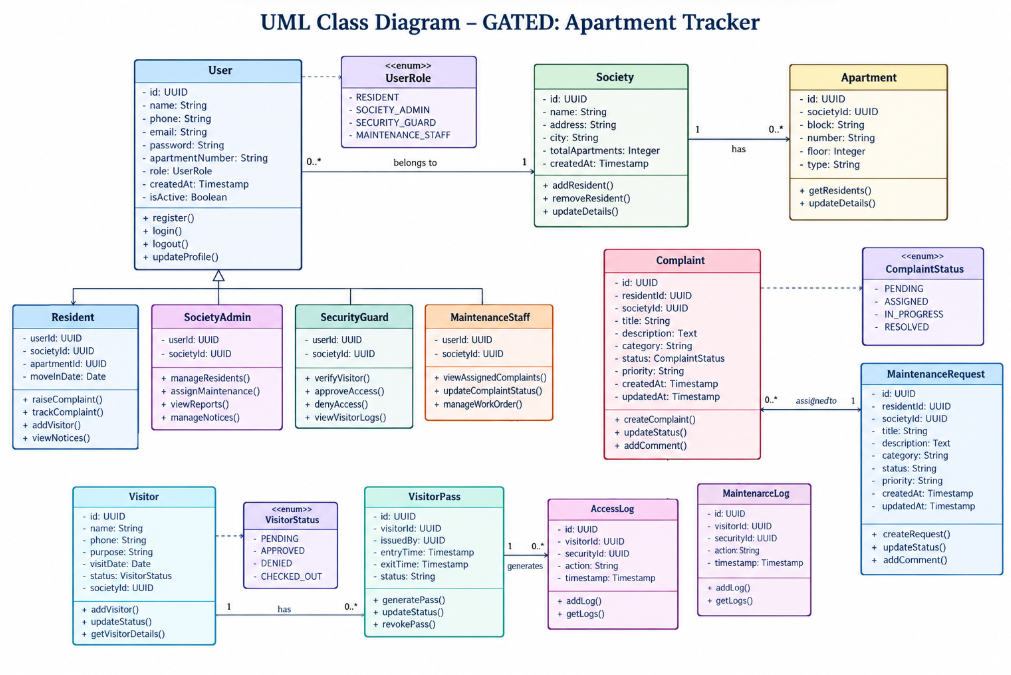
\includegraphics[width=\textwidth]{class_diagram.png}
    \caption{UML Class Diagram}
    \label{fig:class}
\end{figure}

The classes represent users and their roles along with
society, apartment, maintenance, visitor, and access
management functionality.

% ==================================================
% ER DIAGRAM
% ==================================================

\section{Entity Relationship Diagram}

The Entity Relationship (ER) Diagram represents the
database structure of GATED: Apartment Tracker. It
illustrates the major entities, their attributes, and
the relationships between them.

\begin{figure}[H]
    \centering
    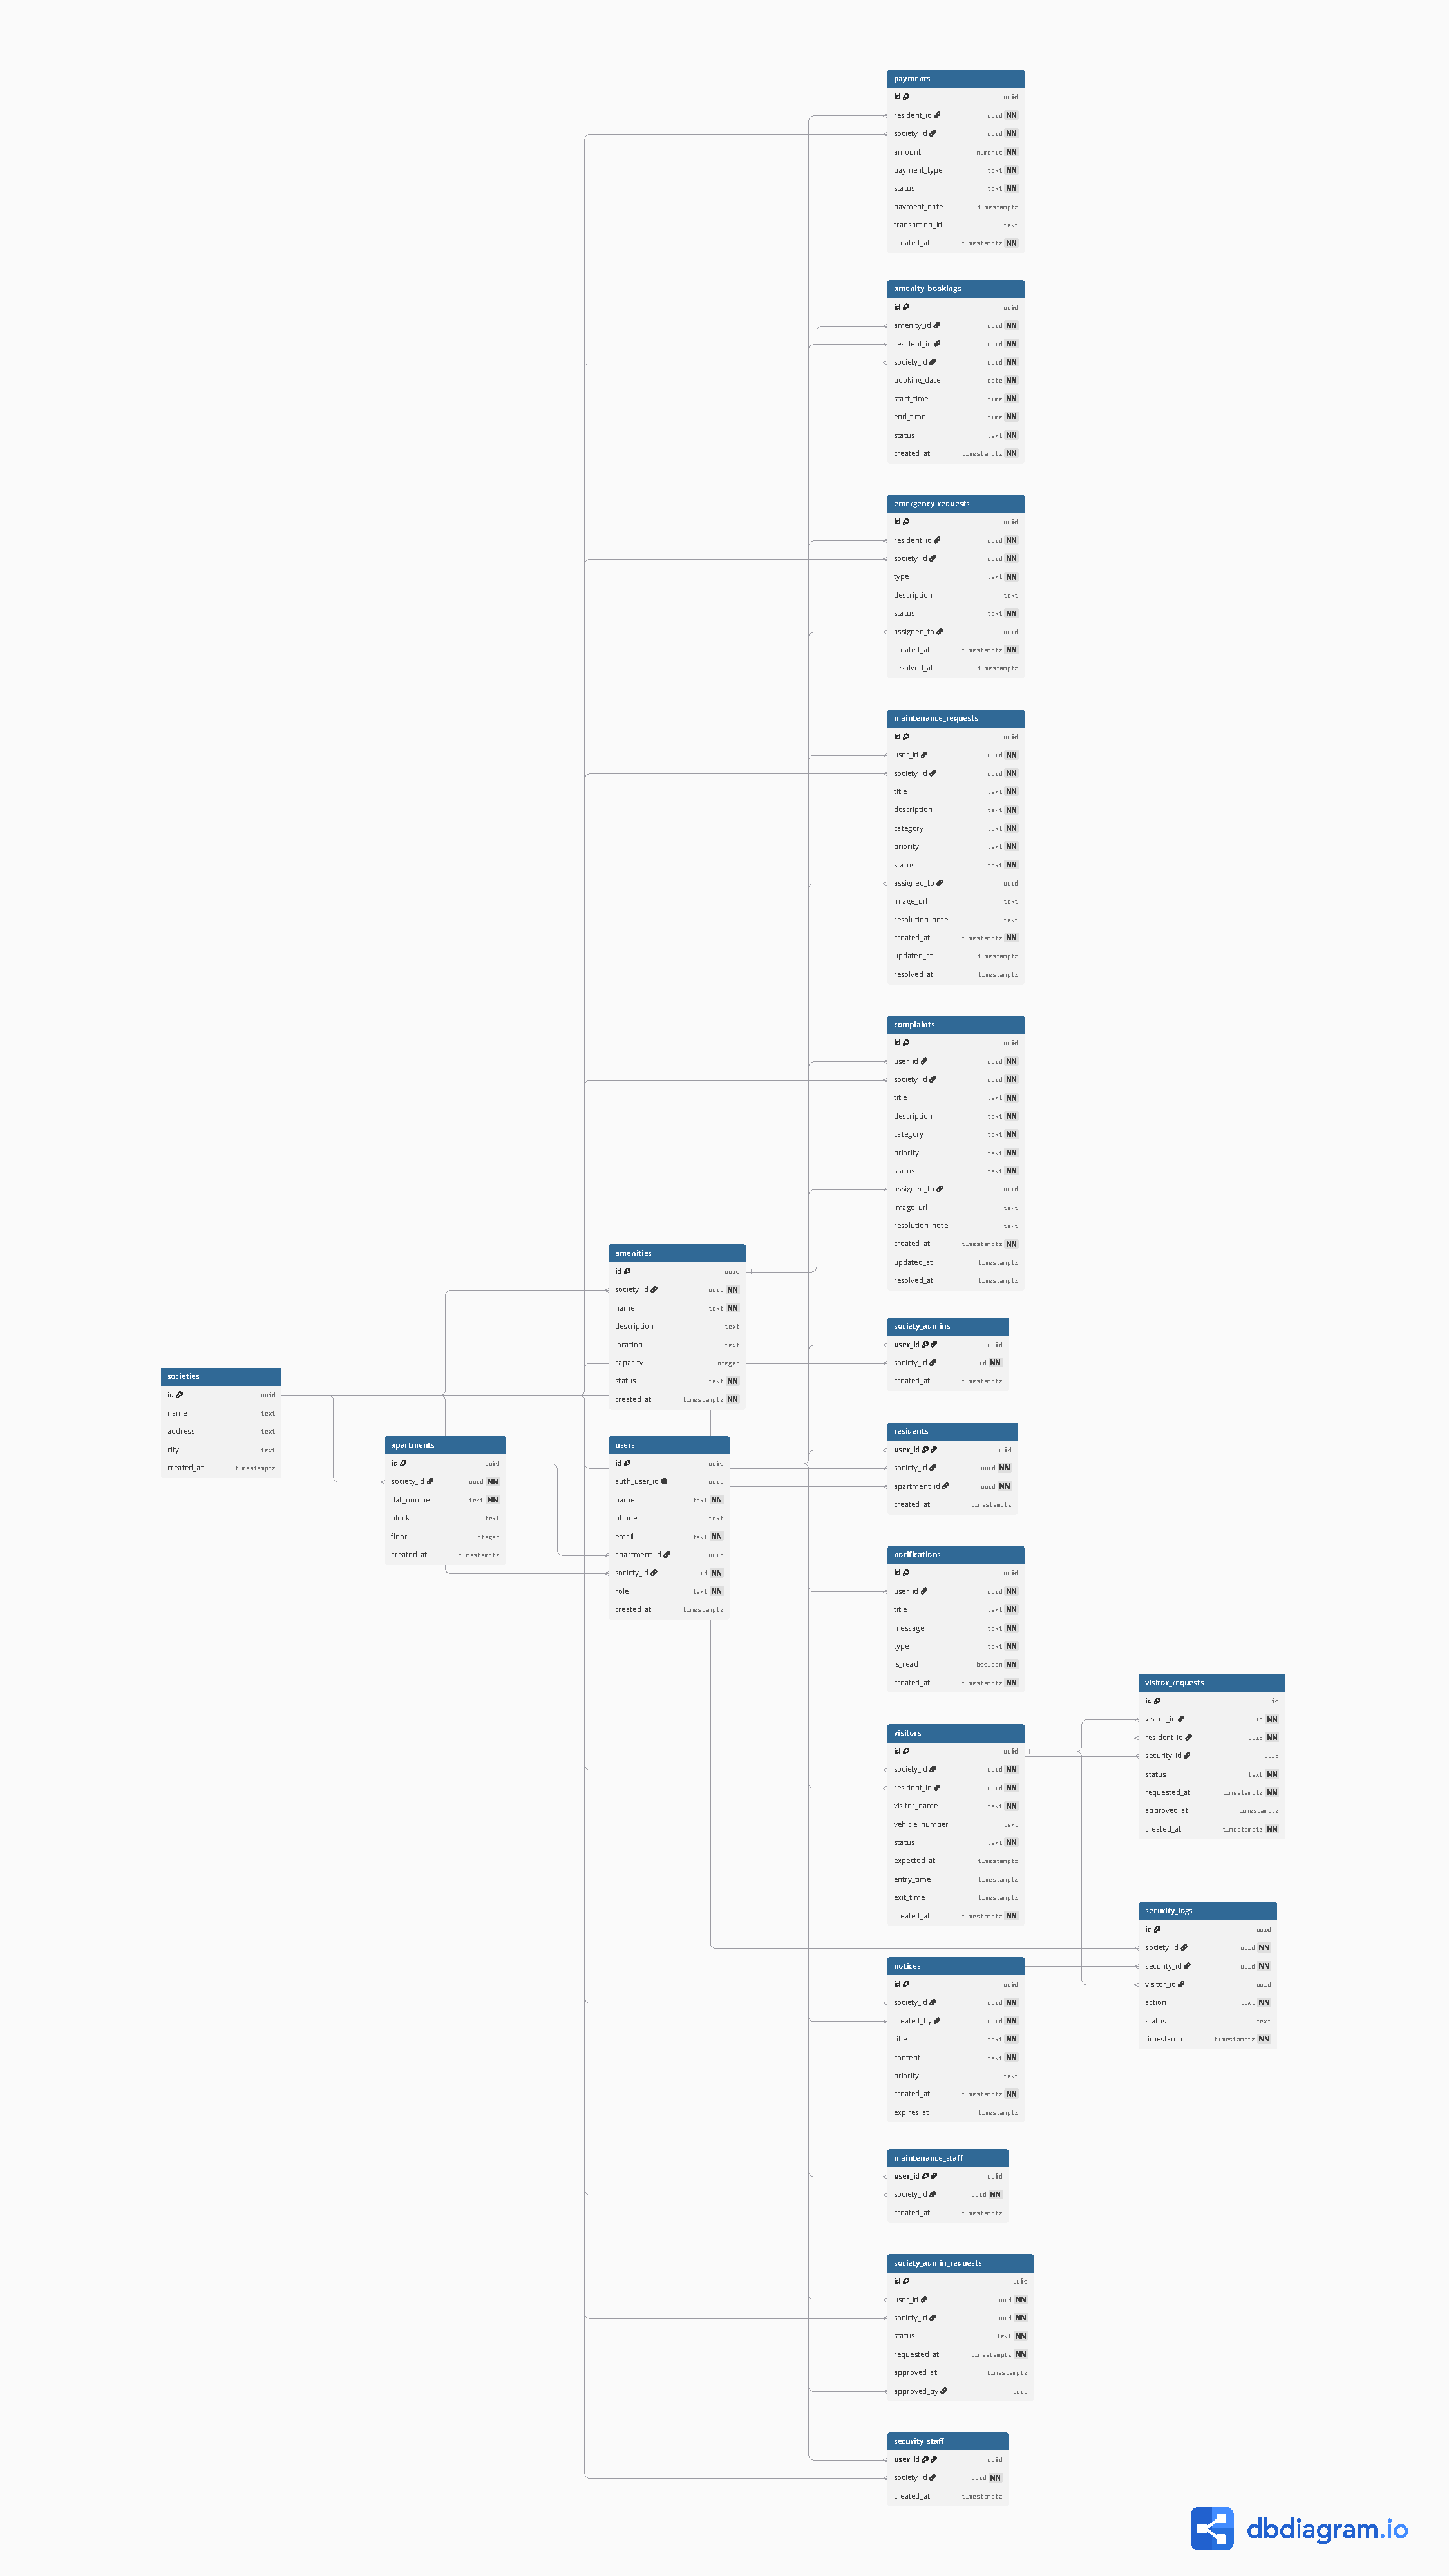
\includegraphics[
        width=\textwidth,
        height=0.75\textheight,
        keepaspectratio
    ]{er_diagram.pdf}
    \caption{Entity Relationship Diagram}
    \label{fig:er}
\end{figure}

The database primarily stores information related to
users, societies, apartments, maintenance requests,
visitors, and visitor passes.

% ==================================================
% UML SEQUENCE DIAGRAM
% ==================================================

\section{UML Sequence Diagram}

The Sequence Diagram represents the interaction between
the resident, mobile application, authentication service,
database, and other system components during the main
application workflow.

\begin{figure}[htbp]
    \centering
    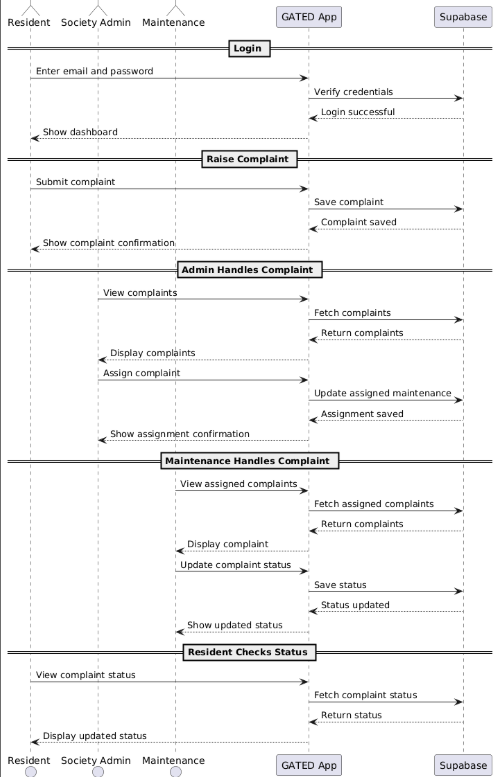
\includegraphics[
        width=\textwidth,
        height=0.75\textheight,
        keepaspectratio
    ]{sequence_diagram.png}
    \caption{UML Sequence Diagram}
    \label{fig:sequence}
\end{figure}

The diagram shows the sequence of interactions involved
in authentication, society selection, role verification,
and access to role-specific functionality. It also
illustrates how requests are processed between the mobile
application and the backend services.

% ==================================================
% TECHNICAL STACK
% ==================================================

\section{Technical Stack}

\begin{itemize}
    \item \textbf{Framework:} React Native with Expo
    \item \textbf{Languages:} JavaScript and TypeScript
    \item \textbf{Database:} PostgreSQL through Supabase
    \item \textbf{Backend:} Supabase
    \item \textbf{Authentication:} Supabase Authentication
    \item \textbf{Navigation:} Expo Router
    \item \textbf{Development Tools:} Visual Studio Code,
    Expo Go, Git and GitHub
    \item \textbf{Security:} Supabase Row Level Security
\end{itemize}

\section{Implementation}

\subsection{Authentication and Role Management}

The authentication module provides secure registration and
login functionality using Supabase Authentication. During
registration, residents provide their name, phone number,
email address, apartment number, and password. The
authentication system verifies the user's credentials and
allows only authenticated users to access the application.

After successful login, the user selects their registered
society. The system then retrieves the user's role and
directs them to the appropriate dashboard. Role-based
access ensures that each type of user can access only the
features relevant to their responsibilities.

The supported roles are:

\begin{itemize}
    \item \textbf{Resident:} Can manage their profile,
    raise complaints, track maintenance requests, and
    manage visitor-related activities.

    \item \textbf{Society Admin:} Can oversee residents,
    complaints, maintenance activities, and other
    society-level operations.

    \item \textbf{Security Guard:} Can verify visitors
    and manage visitor entry and access within the
    society.

    \item \textbf{Maintenance Staff:} Can view assigned
    complaints, work on maintenance issues, and update
    their status.
\end{itemize}

\subsection{Complaint and Maintenance Management}

The Complaint and Maintenance Management module provides
a structured system for reporting and resolving
maintenance-related issues. Residents can raise a
complaint by providing details such as the complaint
title, description, category, and other relevant
information.

Once submitted, each complaint is stored in the database
and associated with the resident who created it. This
allows the complaint to be tracked throughout its
lifecycle. The system maintains different statuses such
as \textit{Pending}, \textit{Assigned}, \textit{In
Progress}, and \textit{Resolved}.

Society administrators can view submitted complaints and
assign them to the appropriate maintenance staff.
Maintenance personnel can then view the complaints
assigned to them, work on the reported issue, and update
its status as the work progresses.

Residents can track the current status of their
complaints, providing transparency about whether an issue
has been received, assigned, is being worked on, or has
been resolved. This reduces dependency on phone calls and
messaging applications for following up on complaints.

The system also maintains a record of previous complaints,
which can help administrators monitor recurring issues,
identify common maintenance problems, and improve the
overall maintenance process of the society.

\subsection{Visitor Management}

The Visitor Management module helps manage visitor access
to the apartment society. Residents can provide visitor
information when required, while security personnel can
verify the visitor's details at the society entrance.

Security guards can review the available visitor
information and approve or deny entry according to the
access details provided. This provides a more organized
alternative to maintaining visitor information through
manual registers.

The module also maintains visitor-related records, making
it easier for security personnel and administrators to
monitor visitor activity within the society.

\subsection{Society Administration}

The Society Administration module provides society
administrators with higher-level access to manage
society-related activities. Administrators can oversee
residents, monitor complaints, assign maintenance
requests, and supervise the overall functioning of the
platform.

The administrator dashboard provides a centralized view
of important society operations and helps coordinate
activities between residents, security personnel, and
maintenance staff.

\subsection{Data Security}

Data security is implemented using Supabase
Authentication and Row Level Security (RLS). Authentication
ensures that only registered users can access the
application, while RLS policies restrict database
operations according to the user's role and permissions.

For example, residents should only be able to access
information relevant to their own account and activities,
while maintenance staff can access complaints assigned to
them. Administrative operations are restricted to users
with the appropriate administrative permissions.

This role-based security approach helps prevent
unauthorized access and protects sensitive resident,
society, complaint, and visitor information.
% ==================================================
% CHAPTER 3
% ==================================================

\chapter{Results and Evaluation}

\section{Testing}

The application is tested through functional and
integration testing.

The major workflows tested include:

\begin{itemize}
    \item User registration
    \item User login
    \item Society selection
    \item Role-based navigation
    \item Complaint request creation
    \item Complaint request management
    \item Database operations
    \item Role-based access restrictions
\end{itemize}

\section{Analysis}

The implementation demonstrates that a mobile-based
platform can centralize multiple apartment society
management activities.

The role-based architecture separates the
responsibilities of residents, society administrators,
security guards, and maintenance staff.

Supabase provides authentication and database services,
while Row Level Security provides additional protection
against unauthorized database access.

During development, challenges related to authentication,
database constraints, role assignment, navigation, and
Row Level Security were addressed through iterative
testing and configuration.

% ==================================================
% CHAPTER 4
% ==================================================

\chapter{Conclusion}

\section{Summary}

GATED: Apartment Tracker is a mobile application designed
to simplify and centralize apartment society management.

The system connects residents, society administrators,
security guards, and maintenance staff through a
role-based platform.

The application provides authentication, society
selection, role-based dashboards, maintenance request
management, and visitor access management.

React Native with Expo is used for mobile application
development, while Supabase provides authentication and
database services.

\section{Future Scope}

The system can be further enhanced with:

\begin{enumerate}
    \item Real-time notifications for visitors and
    maintenance requests.

    \item QR-based visitor passes.

    \item Advanced delivery and visitor management.

    \item Emergency alerts and emergency contacts.

    \item Society-wide announcements.

    \item Online maintenance fee and payment management.

    \item Analytics dashboards for administrators.

    \item Support for multiple societies and larger
    numbers of users.
\end{enumerate}

\section{Final Remarks}

GATED: Apartment Tracker demonstrates how mobile
application development and cloud-based backend
services can be used to improve residential society
management.

The proposed system provides a centralized platform for
residents, administrators, security personnel, and
maintenance staff. With further development, the
application can be extended into a comprehensive smart
apartment management solution.

% ==================================================
% BIBLIOGRAPHY
% ==================================================

\printbibliography[heading=bibintoc]

\end{document}
```
